\documentclass[
t, % align text inside frame to t=top, b=bottom, c=center
10pt, % 8pt, 9pt, 10pt, 11pt, 12pt, 14pt, 17pt, 20pt available as text font
aspectratio=1610, % select your aspect ratio 4:3=43, 16:9=169, 16:10=1610
ngerman,
english,
%handout,
]{beamer}
\usetheme{Juelich}

\usepackage{babel}
\usepackage[utf8]{inputenc}
\usepackage[labelfont=bf]{caption}
\usepackage[colorlinks=true, urlcolor=blue]{hyperref}
\usepackage{pdfpages}

\title{Introduction to Version Control}
\subtitle{Time travel for beginners}
\author{Julia Sprenger}
\institute[My Institute]{INM-6/10}
\date{June 29, 2018}
\titlegraphic{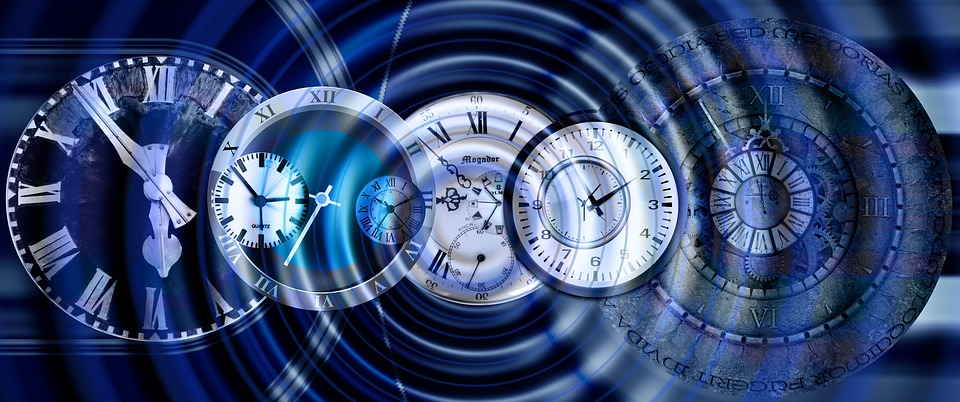
\includegraphics[width=\paperwidth]{graphics/clock-1527693_960_720.jpg}}

\newcommand\blfootnote[1]{%
  \begingroup
  \renewcommand\thefootnote{}\footnote{#1}%
  \addtocounter{footnote}{-1}%
  \endgroup
}

\begin{document}
% only use \maketitle to set your titlepage
\fzjset{title page=image}
\maketitle

% \fzjset{title page=text}
% \maketitle

\part{Why should I care about versions?}
\makepart

\begin{frame}
    \centering
    
\includegraphics[height=\textheight]{graphics/phd101212s.jpg}\\
    \url{http://phdcomics.com/comics.php?f=1531}
\end{frame}

\begin{frame}
    \centering
    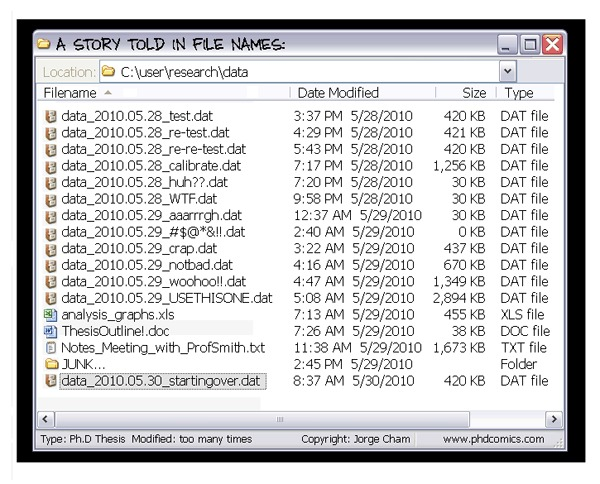
\includegraphics[height=\textheight]{graphics/phd052810s.jpg}\\
    \url{http://phdcomics.com/comics.php?f=1323}
\end{frame}

\begin{frame}
    \frametitle{Version Control using folder and filenames}
    \begin{itemize}[<+->]
        \item only readable by you ...
        \item ... as long as you remember
        \item no consistent structure or naming scheme enforced
        \item no detailed description of changes (why were changes performed?)
        \item no easy way of comparing changes between versions (which changes were performed?)
        \item \hdots{}
    \end{itemize}
\end{frame}

\begin{frame}
    
\includepdf[pages=9, offset=0mm 10mm, scale=0.9]{sources/git-github.pdf}
    \blfootnote{\url{https://github.com/rstudio/webinars/tree/master/06-Collaboration-and-time-travel-version-control}}
\end{frame}

\begin{frame}
    
\includepdf[pages=10, offset=0mm 10mm, scale=0.9]{sources/git-github.pdf}
    \blfootnote{\url{https://github.com/rstudio/webinars/tree/master/06-Collaboration-and-time-travel-version-control}}
\end{frame}

\part{Version Control Systems}
\makepart

\begin{frame}
    \frametitle{Different Version Control Systems}
    \centering
    \vfill
    \begin{tabular}{ c l r }
        
\includegraphics[height=0.8cm]{graphics/giticon_orange.eps} & \large{GIT} &  distributed system\\
        
\includegraphics[height=0.8cm]{graphics/Mercurial_logo.png} & \large{Mercurial} &  distributed system\\
        
\includegraphics[height=0.8cm]{graphics/Subversion_Logo.png} & \large{SVN} &  centralized system\\
    \end{tabular}
    \vfill

\end{frame}

\section{GIT}
\begin{frame}
	\frametitle{GIT}
\end{frame}


\begin{frame}
    \frametitle{GIN}
    \centering
    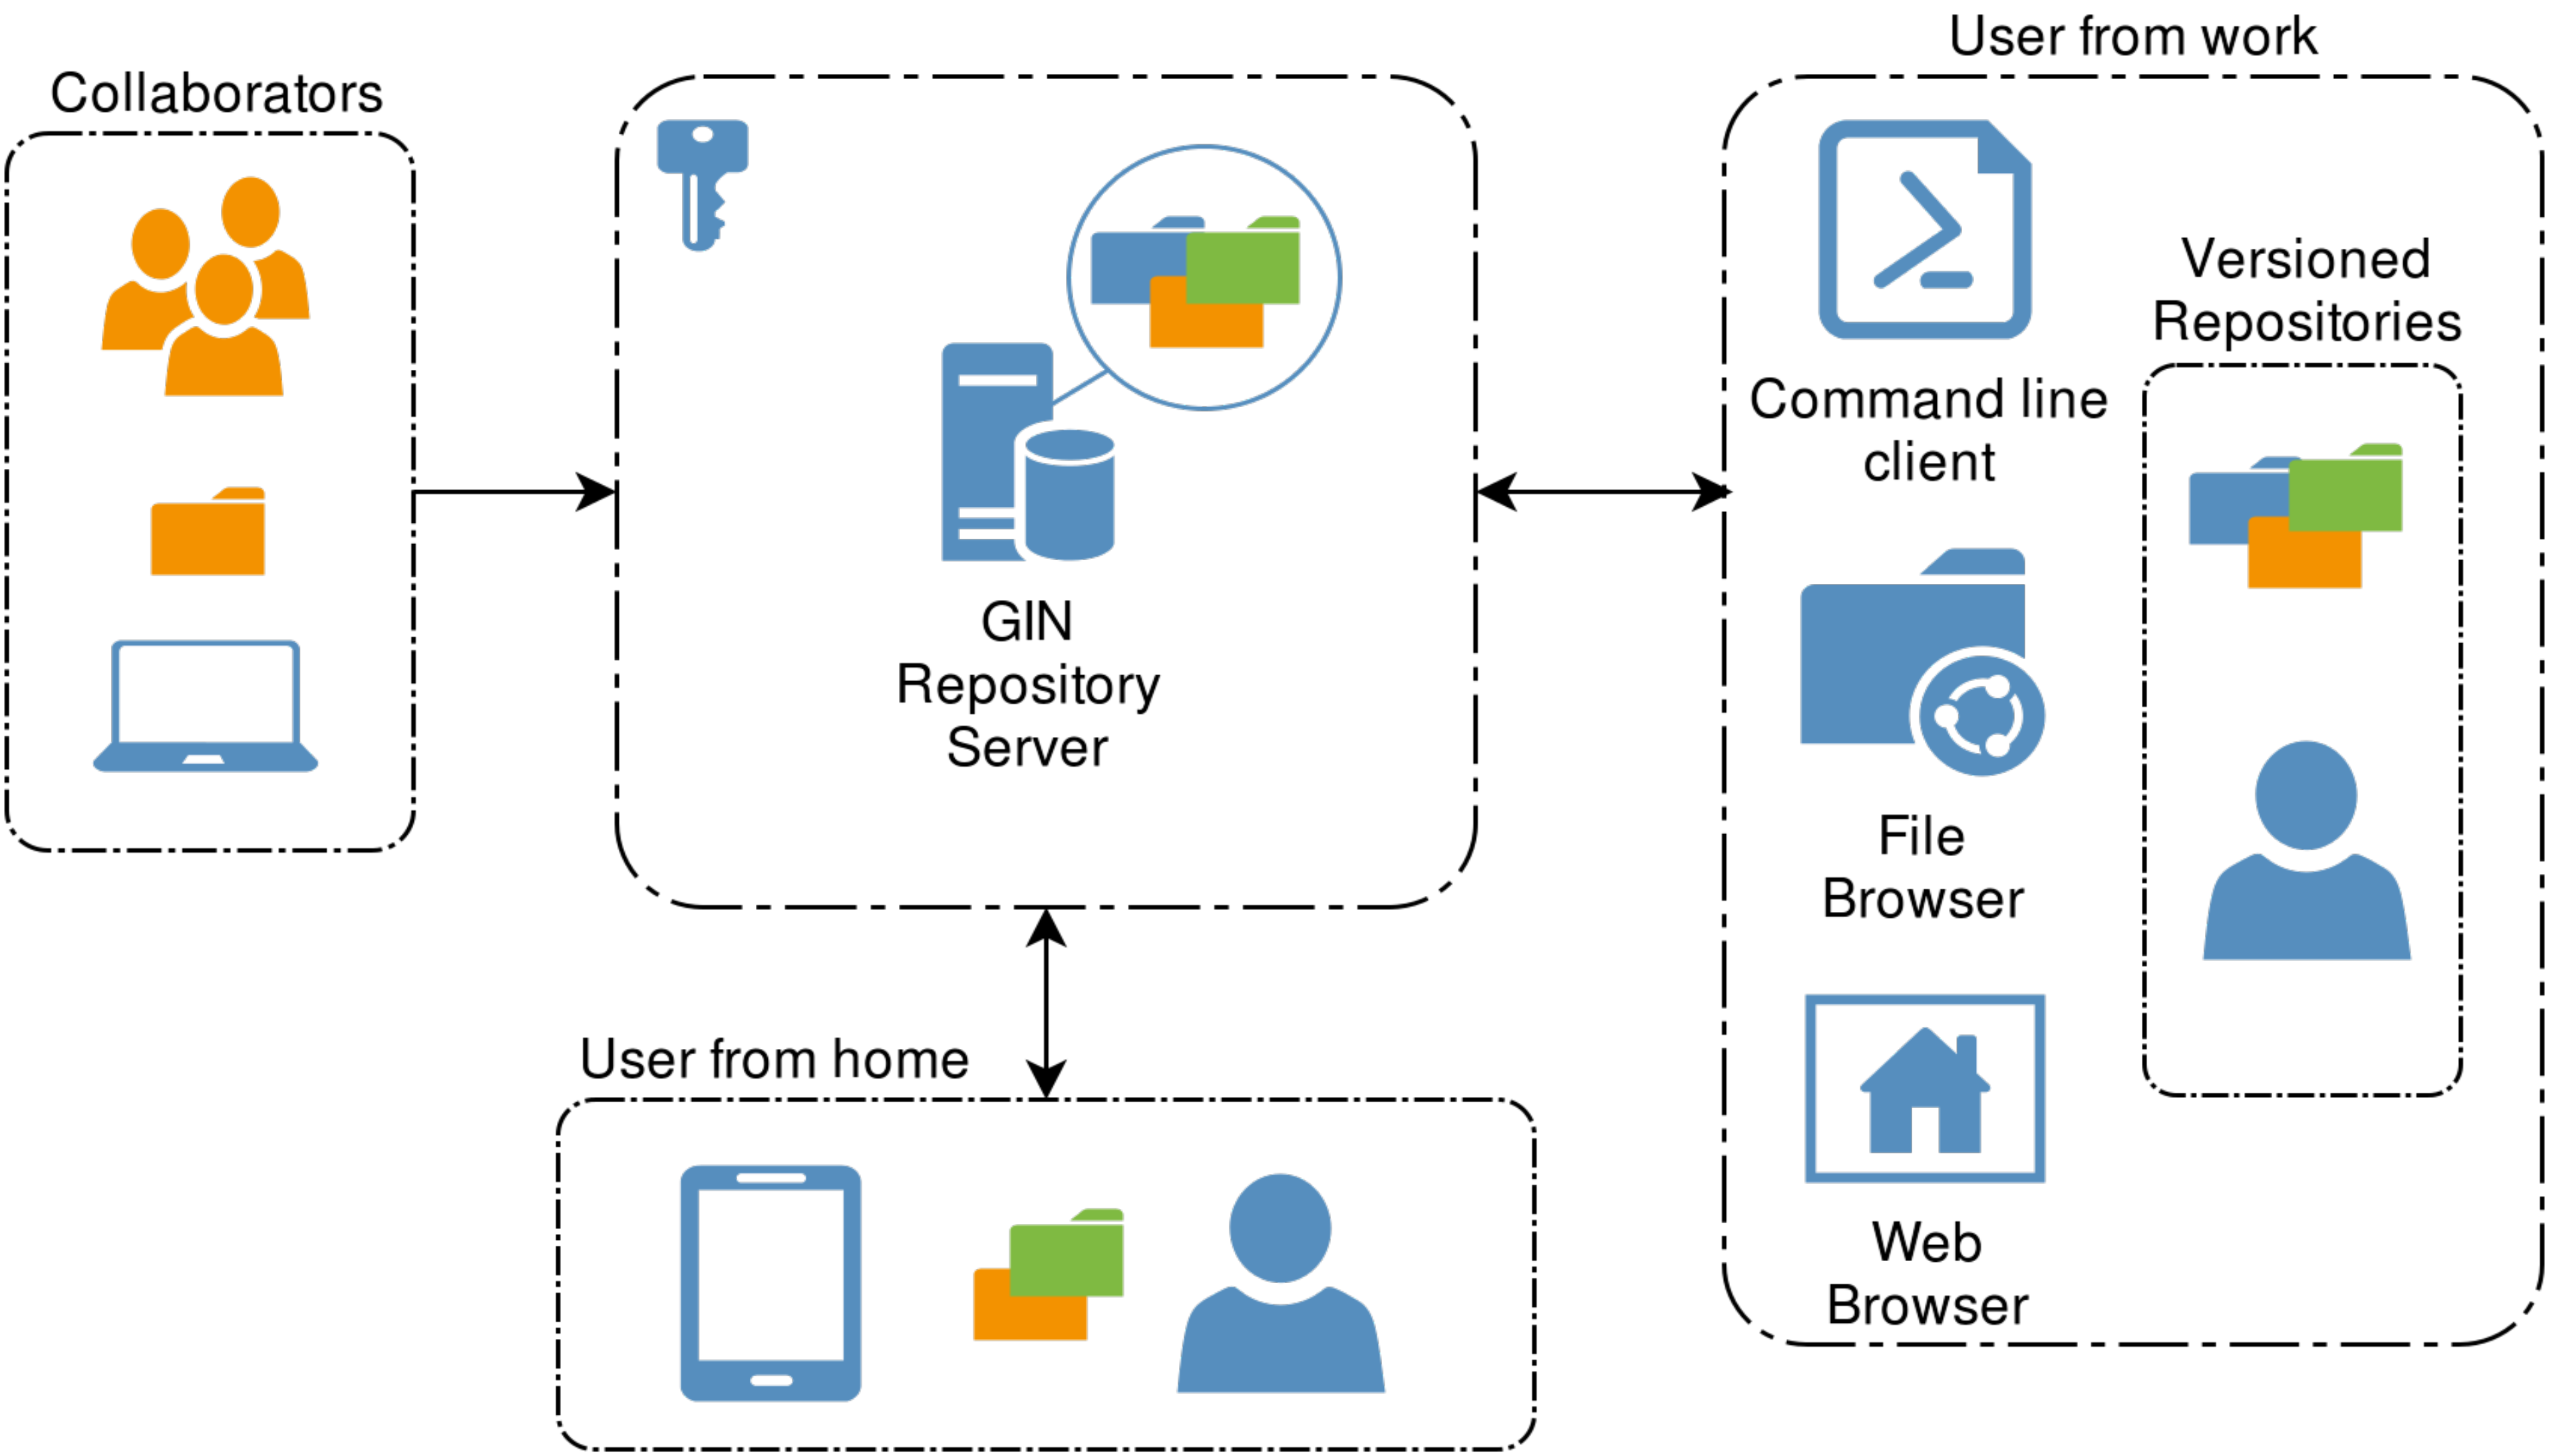
\includegraphics[height=0.7\textheight]{graphics/image9539.png}\\
\end{frame}

\section{Summary}

\begin{frame}
    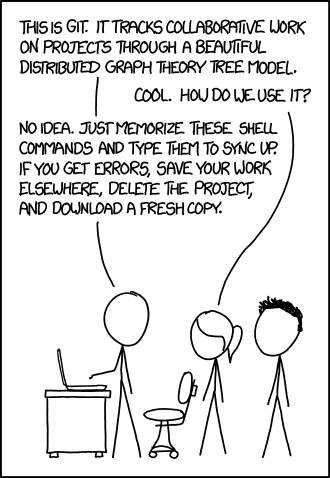
\includegraphics[height=0.7\textheight]{graphics/xkcd-git.png}
    \blfootnote{\url{https://xkcd.com/1597}}
\end{frame}


\begin{frame}
    \frametitle{Thanks for your attention}
    \centering
    
\includegraphics[height=0.7\textheight]{graphics/dn28374-1_800.jpg}\\
    \url{https://www.newscientist.com/article/dn28374-back-to-the-future-does-physics-of-martys-time-travel-add-up/}
\end{frame}


\section{References}
\begin{frame}
    \frametitle{References and further reads}
    This presentation is available at \url{https://github.com/JuliaSprenger/vc_talk}
    Inspiration for this presentation comes from
    \begin{itemize}
        \item Version Control Tutorial \& GIT \newline \url{https://github.com/rstudio/webinars/tree/master/06-Collaboration-and-time-travel-version-control}
        \item iaeie
    \end{itemize}
\end{frame}



\end{document}
